\subsection{Casos de prueba:}

Dado que el algoritmo debe encontrar la división de trabajos que dá el mínimo, las instancias que permiten verificar su correctitud son las siguientes:
\begin{itemize}
\item Hay sólo un trabajo. Ej: 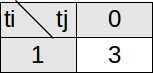
\includegraphics[scale=0.6]{ej1/caso1.png} \\
Solución: t1 en una máquina, la otra libre, costo: 3.\\
El algoritmo dá la solución esperada.
\end{itemize}

El mínimo está dado por la siguiente distribución:
\begin{itemize}
\item Todos los trabajos en una máquina y ninguno en la otra.\\
Ej: 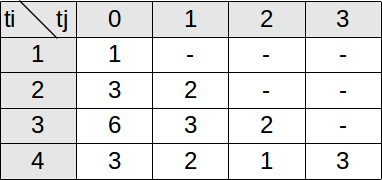
\includegraphics[scale=0.6]{ej1/caso2.png} \\
Solución: t1, t2, t3, t4 en una máquina, la otra libre, costo:8.\\
El algoritmo dá la solución esperada.\\

\item División (en orden) de los trabajos.\\
Ej: 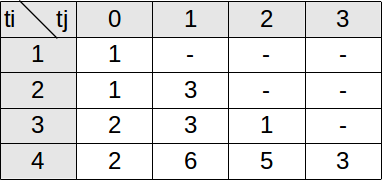
\includegraphics[scale=0.6]{ej1/caso3.png} \\
Solución: t1 en una máquina, t2, t3, t4 en la otra, costo: 6.\\
El algoritmo dá la solución esperada.\\

\item División (sin orden) de los trabajos.\\
Ej: 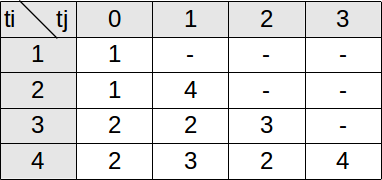
\includegraphics[scale=0.6]{ej1/caso4.png} \\
Solución: t1, t3 en una máquina t2, t4 en la otra, costo: 6.\\
El algoritmo dá la solución esperada.\\
\end{itemize}

Elegimos estos casos porque son distintas formas de distribuir los trabajos, lo que intentamos mostrar es que el algoritmo no deja distribuciones sín mirar.\\